% answers.tex —— 2013 年·湖南卷·文科 · 参考答案与详细解析片段
% 由 tools/generate_projects.py 依来源总账自 2013/2013_数学真题_湖南文_试题.md + 2013/2013_数学真题_湖南文_解析正文.md + 2013/2013_数学真题_湖南文_答案要点.md 生成，勿手改（改源 MD 后重跑）

\begin{answer}
\gksolhead{1}{}

\textbf{题目}：

复数 $z=\mathrm i\cdot(1+\mathrm i)$（$\mathrm i$ 为虚数单位）在复平面上对应的点位于\mbox{（　　）}
（A）第一象限；（B）第二象限；（C）第三象限；（D）第四象限。

\Needspace{4\baselineskip}
\textbf{解析}
\Needspace{5\baselineskip}
由 $\mathrm i^2=-1$ 得
\nopagebreak[4]
\[z=\mathrm i(1+\mathrm i)=\mathrm i+\mathrm i^2=-1+\mathrm i,\]
故 $z$ 对应的点为 $(-1,1)$，位于第二象限。选 B。

\gkanswer{答案：B。}

\end{answer}
\begin{answer}
\gksolhead{2}{}

\textbf{题目}：

“$1<x<2$”是“$x<2$”成立的\mbox{（　　）}
（A）充分不必要条件；（B）必要不充分条件；（C）充分必要条件；（D）既不充分也不必要条件。

\Needspace{4\baselineskip}
\textbf{解析}
若 $1<x<2$，则必有 $x<2$，故“$1<x<2$”是“$x<2$”的充分条件。
反之，取 $x=0$，它满足 $x<2$，但不满足 $1<x<2$，故不是必要条件。
所以“$1<x<2$”是“$x<2$”的充分不必要条件。选 A。

\gkanswer{答案：A。}

\end{answer}
\begin{answer}
\gksolhead{3}{}

\textbf{题目}：

某工厂甲、乙、丙三个车间生产了同一种产品，数量分别为 $120$ 件，$80$ 件，$60$ 件。为了解它们的产品质量是否存在显著差异，用分层抽样方法抽取了一个容量为 $n$ 的样本进行调查，其中从丙车间的产品中抽取了 $3$ 件，则 $n=$\mbox{（　　）}
（A）$9$；（B）$10$；（C）$12$；（D）$13$。

\Needspace{4\baselineskip}
\textbf{解析}
\Needspace{5\baselineskip}
三个车间的产品总数为
\nopagebreak[4]
\[120+80+60=260.\]
\Needspace{5\baselineskip}
分层抽样按比例抽取，故样本容量 $n$ 与总数之比等于丙车间被抽数量与丙车间产品数之比：
\nopagebreak[4]
\[\frac{n}{260}=\frac3{60},\]
\Needspace{5\baselineskip}
解得
\nopagebreak[4]
\[n=260\times\frac3{60}=13.\]
选 D。

\gkanswer{答案：D。}

\end{answer}
\begin{answer}
\gksolhead{4}{}

\textbf{题目}：

已知 $f(x)$ 是奇函数，$g(x)$ 是偶函数，且 $f(-1)+g(1)=2$，$f(1)+g(-1)=4$，则 $g(1)$ 等于\mbox{（　　）}
（A）$4$；（B）$3$；（C）$2$；（D）$1$。

\Needspace{4\baselineskip}
\textbf{解析}
\Needspace{5\baselineskip}
由 $f(x)$ 为奇函数得 $f(-1)=-f(1)$；由 $g(x)$ 为偶函数得 $g(-1)=g(1)$。于是两式化为
\nopagebreak[4]
\[-f(1)+g(1)=2,\qquad f(1)+g(1)=4.\]
\Needspace{5\baselineskip}
两式相加消去 $f(1)$：
\nopagebreak[4]
\[2g(1)=6\implies g(1)=3.\]
选 B。

\gkanswer{答案：B。}

\end{answer}
\begin{answer}
\gksolhead{5}{}

\textbf{题目}：

在锐角 $\triangle ABC$ 中，角 $A$，$B$ 所对的边长分别为 $a$，$b$。若 $2a\sin B=\sqrt3b$，则角 $A$ 等于\mbox{（　　）}
（A）$\dfrac\pi3$；（B）$\dfrac\pi4$；（C）$\dfrac\pi6$；（D）$\dfrac\pi{12}$。

\Needspace{4\baselineskip}
\textbf{解析}
\Needspace{5\baselineskip}
由正弦定理 $\dfrac a{\sin A}=\dfrac b{\sin B}$ 得 $a=\dfrac{b\sin A}{\sin B}$。代入已知式：
\nopagebreak[4]
\[2\cdot\frac{b\sin A}{\sin B}\cdot\sin B=\sqrt3b.\]
\Needspace{5\baselineskip}
因 $b>0$，$\sin B>0$，约去 $b\sin B$ 得
\nopagebreak[4]
\[2\sin A=\sqrt3\implies\sin A=\frac{\sqrt3}2.\]
\Needspace{5\baselineskip}
又 $\triangle ABC$ 为锐角三角形，故
\nopagebreak[4]
\[A=\frac\pi3.\]
选 A。

\gkanswer{答案：A。}

\end{answer}
\begin{answer}
\gksolhead{6}{}

\textbf{题目}：

函数 $f(x)=\ln x$ 的图象与函数 $g(x)=x^2-4x+4$ 的图象的交点个数为\mbox{（　　）}
（A）$0$；（B）$1$；（C）$2$；（D）$3$。

\Needspace{4\baselineskip}
\textbf{解析}
\Needspace{5\baselineskip}
交点个数即方程
\nopagebreak[4]
\[\ln x=x^2-4x+4=(x-2)^2\]
\Needspace{5\baselineskip}
在 $x>0$ 上的实根个数。令
\nopagebreak[4]
\[h(x)=\ln x-(x-2)^2.\]
\Needspace{5\baselineskip}
取点判断符号：
\nopagebreak[4]
\[h(1)=0-1=-1<0,\quad h(2)=\ln2-0>0,\quad h(3)=\ln3-1>0,\quad h(4)=\ln4-4<0.\]
由 $h(1)<0<h(2)$ 知 $(1,2)$ 内有零点；由 $h(3)>0>h(4)$ 知 $(3,4)$ 内有零点。
再看根的个数：$h''(x)=-\dfrac1{x^2}-2<0$，故 $h'(x)=\dfrac1x-2x+4$ 在 $(0,+\infty)$ 上严格递减，$h$ 至多有一个极大值点，从而 $h$ 的零点至多两个，每个零点两侧符号必相反。
所以 $h$ 恰有两个零点，两图象的交点个数为 $2$。选 C。

\gkanswer{答案：C。}

\end{answer}
\begin{answer}
\gksolhead{7}{}

\textbf{题目}：

已知正方体的棱长为 $1$，其俯视图是一个面积为 $1$ 的正方形，侧视图是一个面积为 $\sqrt2$ 的矩形，则该正方体的正视图的面积等于\mbox{（　　）}
（A）$\dfrac{\sqrt3}2$；（B）$1$；（C）$\dfrac{\sqrt2+1}2$；（D）$\sqrt2$。

\Needspace{4\baselineskip}
\textbf{解析}
正方体棱长为 $1$，俯视图是面积为 $1$ 的正方形，说明俯视图恰为棱长为 $1$ 的正方形，且正视图、侧视图的高都等于 $1$。
\Needspace{5\baselineskip}
设俯视图中正方形的一条边与正视图方向成角 $\theta$，则该正方形在两个互相垂直的水平方向上的投影宽度分别为
\nopagebreak[4]
\[|\cos\theta|+|\sin\theta|,\qquad|\sin\theta|+|\cos\theta|,\]
两者相等。故正视图与侧视图的宽相等。
\Needspace{5\baselineskip}
已知侧视图是面积为 $\sqrt2$ 的矩形，其高为 $1$，故宽为 $\sqrt2$；于是正视图也是宽 $\sqrt2$、高 $1$ 的矩形，面积为
\nopagebreak[4]
\[S=\sqrt2\times1=\sqrt2.\]
选 D。

\gkanswer{答案：D。}

\end{answer}
\begin{answer}
\gksolhead{8}{}

\textbf{题目}：

已知 $\boldsymbol a$，$\boldsymbol b$ 是单位向量，$\boldsymbol a\cdot\boldsymbol b=0$。若向量 $\boldsymbol c$ 满足 $|\boldsymbol c-\boldsymbol a-\boldsymbol b|=1$，则 $|\boldsymbol c|$ 的最大值为\mbox{（　　）}
（A）$\sqrt2-1$；（B）$\sqrt2$；（C）$\sqrt2+1$；（D）$\sqrt2+2$。

\Needspace{4\baselineskip}
\textbf{解析}
\Needspace{5\baselineskip}
由 $\boldsymbol a\perp\boldsymbol b$，$|\boldsymbol a|=|\boldsymbol b|=1$ 得
\nopagebreak[4]
\[|\boldsymbol a+\boldsymbol b|=\sqrt{|\boldsymbol a|^2+|\boldsymbol b|^2}=\sqrt2.\]
\Needspace{5\baselineskip}
条件 $|\boldsymbol c-\boldsymbol a-\boldsymbol b|=1$ 表示 $\boldsymbol c$ 的终点在以 $\boldsymbol a+\boldsymbol b$ 的终点为圆心、$1$ 为半径的圆上。由三角不等式，
\nopagebreak[4]
\[|\boldsymbol c|\leqslant|\boldsymbol a+\boldsymbol b|+1=\sqrt2+1,\]
且当 $\boldsymbol c$ 与 $\boldsymbol a+\boldsymbol b$ 同向、$\boldsymbol c=(\sqrt2+1)\dfrac{\boldsymbol a+\boldsymbol b}{|\boldsymbol a+\boldsymbol b|}$ 时取等号。故 $|\boldsymbol c|$ 的最大值为 $\sqrt2+1$。选 C。

\gkanswer{答案：C。}

\end{answer}
\begin{answer}
\gksolhead{9}{}

\textbf{题目}：

已知事件“在矩形 $ABCD$ 的边 $CD$ 上随机取一点 $P$，使 $\triangle APB$ 的最大边是 $AB$”发生的概率为 $\dfrac12$，则 $\dfrac{AD}{AB}=$\mbox{（　　）}
（A）$\dfrac12$；（B）$\dfrac14$；（C）$\dfrac{\sqrt3}2$；（D）$\dfrac{\sqrt7}4$。

\Needspace{4\baselineskip}
\textbf{解析}
\Needspace{5\baselineskip}
设 $AB=a$，$AD=b$，在 $CD$ 上取 $P$，令 $DP=x$（$0\leqslant x\leqslant a$），则 $PC=a-x$，且
\nopagebreak[4]
\[AP^2=x^2+b^2,\qquad PB^2=(a-x)^2+b^2.\]
\Needspace{5\baselineskip}
“$\triangle APB$ 的最大边是 $AB$”等价于 $AP\leqslant AB$ 且 $PB\leqslant AB$，即
\nopagebreak[4]
\[x^2+b^2\leqslant a^2,\qquad(a-x)^2+b^2\leqslant a^2.\]
\Needspace{5\baselineskip}
两式分别给出
\nopagebreak[4]
\[x\leqslant\sqrt{a^2-b^2},\qquad x\geqslant a-\sqrt{a^2-b^2}.\]
\Needspace{5\baselineskip}
故满足条件的 $x$ 构成区间
\nopagebreak[4]
\[\left[a-\sqrt{a^2-b^2},\ \sqrt{a^2-b^2}\right],\]
\Needspace{5\baselineskip}
其长度为 $2\sqrt{a^2-b^2}-a$。由几何概型，
\nopagebreak[4]
\[\frac{2\sqrt{a^2-b^2}-a}{a}=\frac12,\]
\Needspace{5\baselineskip}
即
\nopagebreak[4]
\[2\sqrt{a^2-b^2}=\frac32a\implies a^2-b^2=\frac9{16}a^2\implies b^2=\frac7{16}a^2.\]
\Needspace{5\baselineskip}
故
\nopagebreak[4]
\[\frac{AD}{AB}=\frac ba=\frac{\sqrt7}4.\]
选 D。

\gkanswer{答案：D。}

\end{answer}
\begin{answer}
\gksolhead{10}{}

\textbf{题目}：

已知集合 $U=\{2,3,6,8\}$，$A=\{2,3\}$，$B=\{2,6,8\}$，则 $(\complement_U A)\cap B=$\gkblank{}。

\Needspace{4\baselineskip}
\textbf{解析}
\Needspace{5\baselineskip}
全集 $U=\{2,3,6,8\}$，$A=\{2,3\}$，故
\nopagebreak[4]
\[\complement_U A=\{6,8\}.\]
\Needspace{5\baselineskip}
又 $B=\{2,6,8\}$，所以
\nopagebreak[4]
\[(\complement_U A)\cap B=\{6,8\}\cap\{2,6,8\}=\{6,8\}.\]

\gkanswer{答案：$\{6,8\}$。}

\end{answer}
\begin{answer}
\gksolhead{11}{}

\textbf{题目}：

\Needspace{5\baselineskip}
在平面直角坐标系 $xOy$ 中，若直线
\nopagebreak[4]
\[l_1:\begin{cases}x=2s+1,\\[2pt] y=s,\end{cases}\quad (s\ \text{\text{为参数}})\]
\Needspace{5\baselineskip}
和直线
\nopagebreak[4]
\[l_2:\begin{cases}x=at,\\[2pt] y=2t-1,\end{cases}\quad (t\ \text{\text{为参数}})\]
平行，则常数 $a$ 的值为\gkblank{}。

\Needspace{4\baselineskip}
\textbf{解析}
\Needspace{5\baselineskip}
$l_1$ 的方向向量为 $(2,1)$，$l_2$ 的方向向量为 $(a,2)$。两直线平行，方向向量共线，故
\nopagebreak[4]
\[\begin{vmatrix}2&1\\ a&2\end{vmatrix}=4-a=0,\]
\Needspace{5\baselineskip}
解得
\nopagebreak[4]
\[a=4.\]

\gkanswer{答案：$4$。}

\end{answer}
\begin{answer}
\gksolhead{12}{}

\textbf{题目}：

执行如图所示的程序框图，如果输入 $a=1$，$b=2$，则输出的 $a$ 的值为\gkblank{}。
\nopagebreak[4]
\begin{center}% 2013 湖南卷文科第 12 题：程序框图。
\begin{tikzpicture}[font=\footnotesize, >=Stealth, line width=0.45pt,
  node distance=4.6mm,
  box/.style={draw, minimum height=1.7em, inner xsep=6pt},
  term/.style={draw, rounded corners=5pt, minimum height=1.7em, inner xsep=8pt},
  io/.style={draw, trapezium, trapezium left angle=70, trapezium right angle=110,
             minimum height=1.7em, inner xsep=6pt},
  dec/.style={draw, diamond, aspect=2.2, inner sep=1pt}]
  \node[term] (start) {开始};
  \node[io, below=5mm of start] (input) {输入 $a$，$b$};
  \node[dec, below=5.5mm of input] (cond) {$a>8$?};
  \node[io, right=10mm of cond] (output) {输出 $a$};
  \node[term, below=5mm of output] (end) {结束};
  \node[box, below=6mm of cond] (add) {$a=a+b$};
  \draw[->] (start) -- (input);
  \draw[->] (input) -- (cond);
  \draw[->] (cond) -- node[above] {是} (output);
  \draw[->] (output) -- (end);
  \draw[->] (cond) -- node[right] {否} (add);
  % 否分支回到判断框之前
  \draw[->] (add.west) -- ++(-1.5,0) |- (cond.west);
\end{tikzpicture}
\end{center}
\nopagebreak[4]
\Needspace{4\baselineskip}
\textbf{解析}
\Needspace{5\baselineskip}
初始 $a=1$，$b=2$。每次判断 $a>8$：不成立则执行 $a=a+b$，成立则输出 $a$。逐次计算：
\nopagebreak[4]
\[a=1\ \to\ 3\ \to\ 5\ \to\ 7\ \to\ 9.\]
当 $a=9$ 时 $9>8$ 成立，输出 $a=9$。故输出的 $a$ 的值为 $9$。

\gkanswer{答案：$9$。}

\end{answer}
\begin{answer}
\gksolhead{13}{}

\textbf{题目}：

\Needspace{5\baselineskip}
若变量 $x$，$y$ 满足约束条件
\nopagebreak[4]
\[\begin{cases}x+2y\leqslant8,\\[2pt] 0\leqslant x\leqslant4,\\[2pt] 0\leqslant y\leqslant3,\end{cases}\]
则 $x+y$ 的最大值为\gkblank{}。

\Needspace{4\baselineskip}
\textbf{解析}
\Needspace{5\baselineskip}
作出可行域，其顶点为
\nopagebreak[4]
\[(0,0),\quad(4,0),\quad(4,2),\quad(2,3),\quad(0,3).\]
其中 $(4,2)$ 是 $x=4$ 与 $x+2y=8$ 的交点，$(2,3)$ 是 $y=3$ 与 $x+2y=8$ 的交点。
\Needspace{5\baselineskip}
在各顶点处计算 $z=x+y$：
\nopagebreak[4]
\[0,\quad4,\quad6,\quad5,\quad3.\]
故 $x+y$ 的最大值为 $6$（在 $(4,2)$ 处取得）。

\gkanswer{答案：$6$。}

\end{answer}
\begin{answer}
\gksolhead{14}{}

\textbf{题目}：

设 $F_1$，$F_2$ 是双曲线 $C:\dfrac{x^2}{a^2}-\dfrac{y^2}{b^2}=1$（$a>0$，$b>0$）的两个焦点。若在 $C$ 上存在一点 $P$，使 $PF_1\perp PF_2$，且 $\angle PF_1F_2=30^\circ$，则 $C$ 的离心率为\gkblank{}。

\Needspace{4\baselineskip}
\textbf{解析}
\Needspace{5\baselineskip}
由 $PF_1\perp PF_2$ 知 $\triangle PF_1F_2$ 是以 $F_1F_2=2c$ 为斜边的直角三角形。又 $\angle PF_1F_2=30^\circ$，故
\nopagebreak[4]
\[PF_2=2c\sin30^\circ=c,\qquad PF_1=2c\cos30^\circ=\sqrt3c.\]
\Needspace{5\baselineskip}
点 $P$ 在双曲线右支上（$PF_1>PF_2$），由双曲线定义
\nopagebreak[4]
\[PF_1-PF_2=2a,\]
\Needspace{5\baselineskip}
即
\nopagebreak[4]
\[(\sqrt3-1)c=2a\implies e=\frac ca=\frac2{\sqrt3-1}=\sqrt3+1.\]
故离心率为 $\sqrt3+1$。

\gkanswer{答案：$\sqrt3+1$。}

\end{answer}
\begin{answer}
\gksolhead{15}{}

\textbf{题目}：

对于 $E=\{a_1,a_2,\cdots,a_{100}\}$ 的子集 $X=\{a_{i_1},a_{i_2},\cdots,a_{i_k}\}$，定义 $X$ 的“特征数列”为 $x_1$，$x_2$，$\cdots$，$x_{100}$，其中 $x_{i_1}=x_{i_2}=\cdots=x_{i_k}=1$，其余项均为 $0$。例如：子集 $\{a_2,a_3\}$ 的“特征数列”为 $0,1,1,0,0,\cdots,0$。
（1） 子集 $\{a_1,a_3,a_5\}$ 的“特征数列”的前 $3$ 项和等于\gkblank{}。
（2） 若 $E$ 的子集 $P$ 的“特征数列”$p_1$，$p_2$，$\cdots$，$p_{100}$ 满足 $p_1=1$，$p_i+p_{i+1}=1$，$1\leqslant i\leqslant99$；$E$ 的子集 $Q$ 的“特征数列”$q_1$，$q_2$，$\cdots$，$q_{100}$ 满足 $q_1=1$，$q_j+q_{j+1}+q_{j+2}=1$，$1\leqslant j\leqslant98$，则 $P\cap Q$ 的元素个数为\gkblank{}。

\Needspace{4\baselineskip}
\textbf{解析}
\Needspace{5\baselineskip}
\textbf{（1）} 子集 $\{a_1,a_3,a_5\}$ 的“特征数列”为 $1,0,1,0,1,0,\cdots$，前 $3$ 项为 $1,0,1$，和为
\nopagebreak[4]
\[1+0+1=2.\]
\Needspace{5\baselineskip}
\textbf{（2）} 由 $p_1=1$，$p_i+p_{i+1}=1$ 依次得
\nopagebreak[4]
\[p_2=0,\ p_3=1,\ p_4=0,\ \cdots,\]
\Needspace{5\baselineskip}
即 $p_i=1$ 当且仅当 $i$ 为奇数。故
\nopagebreak[4]
\[P=\{a_1,a_3,a_5,\cdots,a_{99}\},\]
共 $50$ 个元素。
\Needspace{5\baselineskip}
由 $q_1=1$，$q_1+q_2+q_3=1$ 得 $q_2=q_3=0$；再由 $q_2+q_3+q_4=1$ 得 $q_4=1$，如此循环，得“特征数列”以 $1,0,0$ 为周期。故 $q_i=1$ 当且仅当 $i\equiv1\pmod 3$，
\nopagebreak[4]
\[Q=\{a_1,a_4,a_7,\cdots,a_{100}\},\]
共 $\dfrac{100-1}3+1=34$ 个元素。
\Needspace{5\baselineskip}
于是 $a_i\in P\cap Q$ 当且仅当 $i$ 为奇数且 $i\equiv1\pmod3$，即
\nopagebreak[4]
\[i\equiv1\pmod6.\]
\Needspace{5\baselineskip}
这样的 $i$ 为 $1,7,13,\cdots,97$，个数为
\nopagebreak[4]
\[\frac{97-1}6+1=17.\]
故 $P\cap Q$ 的元素个数为 $17$。

\gkanswer{答案（1）：$2$。}

\gkanswer{答案（2）：$17$。}

\end{answer}
\begin{answer}
\gksolhead{16}{}

\textbf{题目}：

已知函数 $f(x)=\cos x\cdot\cos\left(x-\dfrac\pi3\right)$。
（1） 求 $f\left(\dfrac{2\pi}3\right)$ 的值；
（2） 求使 $f(x)<\dfrac14$ 成立的 $x$ 的取值集合。

\Needspace{4\baselineskip}
\textbf{解析}
\Needspace{5\baselineskip}
由积化和差公式，
\nopagebreak[4]
\[f(x)=\cos x\cos\left(x-\frac\pi3\right)=\frac12\left[\cos\frac\pi3+\cos\left(2x-\frac\pi3\right)\right]=\frac12\cos\left(2x-\frac\pi3\right)+\frac14.\]
\Needspace{5\baselineskip}
\textbf{（1）} 取 $x=\dfrac{2\pi}3$，则 $2x-\dfrac\pi3=\pi$，于是
\nopagebreak[4]
\[f\left(\frac{2\pi}3\right)=\frac12\cos\pi+\frac14=-\frac12+\frac14=-\frac14.\]
\Needspace{5\baselineskip}
\textbf{（2）} 不等式 $f(x)<\dfrac14$ 等价于
\nopagebreak[4]
\[\frac12\cos\left(2x-\frac\pi3\right)<0\iff\cos\left(2x-\frac\pi3\right)<0.\]
\Needspace{5\baselineskip}
故
\nopagebreak[4]
\[2k\pi+\frac\pi2<2x-\frac\pi3<2k\pi+\frac{3\pi}2,\quad k\in\mathbf Z,\]
\Needspace{5\baselineskip}
即
\nopagebreak[4]
\[2k\pi+\frac{5\pi}6<2x<2k\pi+\frac{11\pi}6,\]
\nopagebreak[4]
\[k\pi+\frac{5\pi}{12}<x<k\pi+\frac{11\pi}{12},\quad k\in\mathbf Z.\]
\Needspace{5\baselineskip}
所求集合为
\nopagebreak[4]
\[\left\{x\;\middle|\;k\pi+\frac{5\pi}{12}<x<k\pi+\frac{11\pi}{12},\ k\in\mathbf Z\right\}.\]

\gkanswer{答案（1）：$-\dfrac14$。}

\gkanswer{答案（2）：$\left\{x\;\middle|\;k\pi+\dfrac{5\pi}{12}<x<k\pi+\dfrac{11\pi}{12},\ k\in\mathbf Z\right\}$。}

\end{answer}
\begin{answer}
\gksolhead{17}{}

\textbf{题目}：

如图，在直棱柱 $ABC-A_1B_1C_1$ 中，$\angle BAC=90^\circ$，$AB=AC=\sqrt2$，$AA_1=3$，$D$ 是 $BC$ 的中点，点 $E$ 在棱 $BB_1$ 上运动。
\nopagebreak[4]
\begin{center}% 2013 湖南卷文科第 17 题：直棱柱 ABC-A1B1C1，D 为 BC 中点，E 在 BB1 上。
\begin{tikzpicture}[font=\footnotesize, >=Stealth, line width=0.45pt, scale=1.05]
  \coordinate (B)  at (0,0);
  \coordinate (C)  at (0.5,2.6);
  \coordinate (C1) at (4.1,2.6);
  \coordinate (B1) at (3.6,0);
  \coordinate (D)  at (0.25,1.3);
  \coordinate (A)  at (1.6,0.92);
  \coordinate (A1) at (5.2,0.92);
  \coordinate (E)  at (1.51,0);
  % 前面 BCC1B1
  \draw (B) -- (C) -- (C1) -- (B1) -- cycle;
  % 上底边与 C1E
  \draw (C1) -- (A1);
  \draw (C1) -- (E);
  % 被遮挡的棱
  \draw[dashed] (B) -- (A);
  \draw[dashed] (C) -- (A);
  \draw[dashed] (A) -- (A1);
  \draw[dashed] (A1) -- (B1);
  % 点
  \fill (A) circle (1.4pt) (A1) circle (1.4pt) (B) circle (1.4pt)
        (B1) circle (1.4pt) (C) circle (1.4pt) (C1) circle (1.4pt)
        (D) circle (1.4pt) (E) circle (1.4pt);
  % 标注
  \node[above left]  at (C)  {$C$};
  \node[above right] at (C1) {$C_1$};
  \node[below right] at (A)  {$A$};
  \node[right]       at (A1) {$A_1$};
  \node[below left]  at (B)  {$B$};
  \node[below right] at (B1) {$B_1$};
  \node[left]        at (D)  {$D$};
  \node[below]       at (E)  {$E$};
\end{tikzpicture}
\end{center}
\nopagebreak[4]
（1） 证明：$AD\perp C_1E$；
（2） 当异面直线 $AC$，$C_1E$ 所成的角为 $60^\circ$ 时，求三棱锥 $C_1-A_1B_1E$ 的体积。

\Needspace{4\baselineskip}
\textbf{解析}
\textbf{（1）} 由 $\angle BAC=90^\circ$ 得 $AB\perp AC$；又 $ABC-A_1B_1C_1$ 为直棱柱，故 $AA_1\perp$ 平面 $ABC$，从而 $AB$，$AC$，$AA_1$ 两两垂直。
\Needspace{5\baselineskip}
以 $A$ 为原点，$\overrightarrow{AB}$，$\overrightarrow{AC}$，$\overrightarrow{AA_1}$ 的方向分别为 $x$，$y$，$z$ 轴正方向建立空间直角坐标系。由 $AB=AC=\sqrt2$，$AA_1=3$ 得
\nopagebreak[4]
\[A(0,0,0),\ B(\sqrt2,0,0),\ C(0,\sqrt2,0),\ C_1(0,\sqrt2,3).\]
\Needspace{5\baselineskip}
$D$ 为 $BC$ 的中点，故
\nopagebreak[4]
\[D\left(\frac{\sqrt2}2,\frac{\sqrt2}2,0\right),\]
\Needspace{5\baselineskip}
设 $E(\sqrt2,0,t)$，$0\leqslant t\leqslant3$，则
\nopagebreak[4]
\[\overrightarrow{AD}=\left(\frac{\sqrt2}2,\frac{\sqrt2}2,0\right),\qquad\overrightarrow{C_1E}=(\sqrt2,-\sqrt2,t-3).\]
\Needspace{5\baselineskip}
于是
\nopagebreak[4]
\[\overrightarrow{AD}\cdot\overrightarrow{C_1E}=\frac{\sqrt2}2\cdot\sqrt2+\frac{\sqrt2}2\cdot(-\sqrt2)+0\cdot(t-3)=1-1=0.\]
故 $AD\perp C_1E$。
\Needspace{5\baselineskip}
\textbf{（2）} $\overrightarrow{AC}=(0,\sqrt2,0)$，且
\nopagebreak[4]
\[|\overrightarrow{AC}|=\sqrt2,\qquad|\overrightarrow{C_1E}|=\sqrt{2+2+(t-3)^2}=\sqrt{4+(t-3)^2},\]
\nopagebreak[4]
\[\overrightarrow{AC}\cdot\overrightarrow{C_1E}=-2.\]
\Needspace{5\baselineskip}
异面直线 $AC$，$C_1E$ 所成的角为 $60^\circ$，故
\nopagebreak[4]
\[\frac{|\overrightarrow{AC}\cdot\overrightarrow{C_1E}|}{|\overrightarrow{AC}|\cdot|\overrightarrow{C_1E}|}=\frac2{\sqrt2\sqrt{4+(t-3)^2}}=\frac12.\]
\Needspace{5\baselineskip}
解得
\nopagebreak[4]
\[\sqrt{4+(t-3)^2}=2\sqrt2\implies(t-3)^2=4\implies t=1\ \text{\text{或}}\ t=5.\]
由 $0\leqslant t\leqslant3$ 得 $t=1$，即 $B_1E=BB_1-BE=3-1=2$。
\Needspace{5\baselineskip}
因为 $A_1B_1\parallel AB$，$B_1E$ 在棱 $BB_1$ 上，且 $AB\perp BB_1$，所以 $\triangle A_1B_1E$ 是以 $B_1$ 为直角顶点的直角三角形，
\nopagebreak[4]
\[S_{\triangle A_1B_1E}=\frac12\cdot A_1B_1\cdot B_1E=\frac12\cdot\sqrt2\cdot2=\sqrt2.\]
\Needspace{5\baselineskip}
平面 $A_1B_1E$ 即平面 $ABB_1A_1$，点 $C_1$ 到该平面的距离等于 $AC=\sqrt2$（因 $AC\perp AB$，$AC\perp AA_1$）。故三棱锥体积
\nopagebreak[4]
\[V=\frac13S_{\triangle A_1B_1E}\cdot\sqrt2=\frac13\cdot\sqrt2\cdot\sqrt2=\frac23.\]

\gkanswer{答案（1）：证明见解析。}

\gkanswer{答案（2）：$\dfrac23$。}

\end{answer}
\begin{answer}
\gksolhead{18}{}

\textbf{题目}：

某人在如图所示的直角边长为 $4$ 米的三角形地块的每个格点（指纵、横直线的交叉点以及三角形的顶点）处都种了一株相同品种的作物。根据历年的种植经验，一株该种作物的年收获量 $Y$（单位：kg）与它的“相近”作物株数 $X$ 之间的关系如下表所示：
\nopagebreak[4]
\begin{center}% 2013 湖南卷文科第 18 题：直角边长为 4 的格点三角形地块。
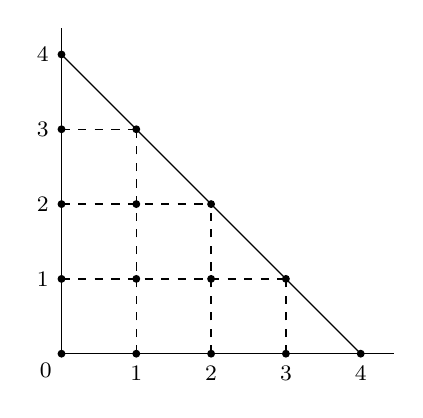
\begin{tikzpicture}[font=\footnotesize, line width=0.45pt, scale=0.95]
  % 坐标轴
  \draw (0,0) -- (4.45,0);
  \draw (0,0) -- (0,4.35);
  % 三角形边界（斜边）
  \draw (0,4) -- (4,0);
  % 三角形内的格线
  \begin{scope}
    \clip (0,0) -- (4,0) -- (0,4) -- cycle;
    \draw[dashed] (0,1) -- (4,1) (0,2) -- (4,2) (0,3) -- (4,3)
                  (1,0) -- (1,4) (2,0) -- (2,4) (3,0) -- (3,4);
  \end{scope}
  % 格点（共 15 个）
  \foreach \x in {0,...,4} {
    \foreach \y in {0,...,4} {
      \pgfmathparse{int(\x+\y<=4)}\ifnum\pgfmathresult=1
        \fill (\x,\y) circle (1.5pt);
      \fi
    }
  }
  % 刻度数字
  \foreach \x in {1,...,4} {
    \node[below] at (\x,-0.04) {$\x$};
  }
  \foreach \y in {1,...,4} {
    \node[left] at (-0.04,\y) {$\y$};
  }
  \node[below left] at (0,0) {$0$};
\end{tikzpicture}
\end{center}
\nopagebreak[4]
\begin{center}
\begin{tabular}{lllll}
\toprule
$X$ & $1$ & $2$ & $3$ & $4$ \\
\midrule
$Y$ & $51$ & $48$ & $45$ & $42$ \\
\bottomrule
\end{tabular}
\end{center}
这里，两株作物“相近”是指它们之间的直线距离不超过 $1$ 米。
（1） 完成下表，并求所种作物的平均年收获量；
\begin{center}
\begin{tabular}{lllll}
\toprule
$Y$ & $51$ & $48$ & $45$ & $42$ \\
\midrule
频数 &  & $4$ &  &  \\
\bottomrule
\end{tabular}
\end{center}
（2） 在所种作物中随机选取一株，求它的年收获量至少为 $48$ kg 的概率。

\Needspace{4\baselineskip}
\textbf{解析}
\textbf{（1）} 格点到另一格点的直线距离不超过 $1$ 米，只可能是与它上下左右相邻的格点（斜对角格点的距离为 $\sqrt2>1$）。故 $X$ 等于该格点在三角形内上下左右相邻格点的个数。
三角形内共 $15$ 个格点，逐个统计（按 $y=0,1,2,3,4$ 分行）：
\begin{itemize}
\item $y=0$：$(0,0)$ 有 $2$ 个，$(1,0)$，$(2,0)$，$(3,0)$ 各有 $3$ 个，$(4,0)$ 有 $1$ 个；
\item $y=1$：$(0,1)$ 有 $3$ 个，$(1,1)$，$(2,1)$ 各有 $4$ 个，$(3,1)$ 有 $2$ 个；
\item $y=2$：$(0,2)$ 有 $3$ 个，$(1,2)$ 有 $4$ 个，$(2,2)$ 有 $2$ 个；
\item $y=3$：$(0,3)$ 有 $3$ 个，$(1,3)$ 有 $2$ 个；
\item $y=4$：$(0,4)$ 有 $1$ 个。
\end{itemize}
于是
\begin{center}
\begin{tabular}{lllll}
\toprule
$X$ & $1$ & $2$ & $3$ & $4$ \\
\midrule
频数 & $2$ & $4$ & $6$ & $3$ \\
\bottomrule
\end{tabular}
\end{center}
对应年收获量 $Y$ 的频数表为
\begin{center}
\begin{tabular}{lllll}
\toprule
$Y$ & $51$ & $48$ & $45$ & $42$ \\
\midrule
频数 & $2$ & $4$ & $6$ & $3$ \\
\bottomrule
\end{tabular}
\end{center}
\Needspace{5\baselineskip}
频数之和 $2+4+6+3=15$，与格点总数一致。平均年收获量为
\nopagebreak[4]
\[\bar Y=\frac{51\times2+48\times4+45\times6+42\times3}{15}=\frac{102+192+270+126}{15}=\frac{690}{15}=46.\]
即所种作物的平均年收获量为 $46$ kg。
\Needspace{5\baselineskip}
\textbf{（2）} 年收获量至少为 $48$ kg 的作物对应 $X=1$ 或 $X=2$，共 $2+4=6$ 株。从 $15$ 株中随机选取一株，所求概率为
\nopagebreak[4]
\[P=\frac6{15}=\frac25.\]

\gkanswer{答案（1）：频数依次为 $2$，$4$，$6$，$3$，平均年收获量为 $46$ kg。}

\gkanswer{答案（2）：$\dfrac25$。}

\end{answer}
\begin{answer}
\gksolhead{19}{}

\textbf{题目}：

设 $S_n$ 为数列 $\{a_n\}$ 的前 $n$ 项和，已知 $a_1\ne0$，$2a_n-a_1=S_1\cdot S_n$，$n\in\mathbf N^*$。
（1） 求 $a_1$，$a_2$，并求数列 $\{a_n\}$ 的通项公式；
（2） 求数列 $\{na_n\}$ 的前 $n$ 项和。

\Needspace{4\baselineskip}
\textbf{解析}
\Needspace{5\baselineskip}
\textbf{（1）} 在 $2a_n-a_1=S_1S_n$ 中令 $n=1$，注意 $S_1=a_1$，得
\nopagebreak[4]
\[2a_1-a_1=a_1^2\implies a_1=a_1^2.\]
\Needspace{5\baselineskip}
因 $a_1\ne0$，故
\nopagebreak[4]
\[a_1=1.\]
\Needspace{5\baselineskip}
于是条件化为
\nopagebreak[4]
\[2a_n-1=S_n. \tag{1}\]
\Needspace{5\baselineskip}
令 $n=2$，得 $2a_2-1=S_2=a_1+a_2=1+a_2$，解得
\nopagebreak[4]
\[a_2=2.\]
\Needspace{5\baselineskip}
对 $n\geqslant2$，将 (1) 与 $2a_{n-1}-1=S_{n-1}$ 相减：
\nopagebreak[4]
\[2a_n-2a_{n-1}=S_n-S_{n-1}=a_n,\]
\Needspace{5\baselineskip}
故
\nopagebreak[4]
\[a_n=2a_{n-1}\quad(n\geqslant2).\]
\Needspace{5\baselineskip}
所以 $\{a_n\}$ 是首项为 $1$、公比为 $2$ 的等比数列，
\nopagebreak[4]
\[a_n=2^{n-1}\quad(n\in\mathbf N^*).\]
\Needspace{5\baselineskip}
\textbf{（2）} 设 $T_n=\displaystyle\sum_{k=1}^n ka_k=\sum_{k=1}^n k\cdot2^{k-1}$，则
\nopagebreak[4]
\[T_n=1+2\cdot2+3\cdot2^2+\cdots+n\cdot2^{n-1},\]
\nopagebreak[4]
\[2T_n=2+2\cdot2^2+3\cdot2^3+\cdots+n\cdot2^n.\]
\Needspace{5\baselineskip}
两式相减：
\nopagebreak[4]
\[T_n=2T_n-T_n=n\cdot2^n-(1+2+2^2+\cdots+2^{n-1})=n\cdot2^n-(2^n-1)=(n-1)2^n+1.\]
故数列 $\{na_n\}$ 的前 $n$ 项和为 $(n-1)2^n+1$。

\gkanswer{答案（1）：$a_1=1$，$a_2=2$，$a_n=2^{n-1}$。}

\gkanswer{答案（2）：$(n-1)2^n+1$。}

\end{answer}
\begin{answer}
\gksolhead{20}{}

\textbf{题目}：

已知 $F_1$，$F_2$ 分别是椭圆 $E:\dfrac{x^2}5+y^2=1$ 的左、右焦点，$F_1$，$F_2$ 关于直线 $x+y-2=0$ 的对称点是圆 $C$ 的一条直径的两个端点。
（1） 求圆 $C$ 的方程；
（2） 设过点 $F_2$ 的直线 $l$ 被椭圆 $E$ 和圆 $C$ 所截得的弦长分别为 $a$，$b$。当 $ab$ 最大时，求直线 $l$ 的方程。

\Needspace{4\baselineskip}
\textbf{解析}
\Needspace{5\baselineskip}
\textbf{（1）} 设点 $(x,y)$ 关于直线 $x+y-2=0$ 的对称点为 $(x',y')$。由中点在该直线上、连线与直线垂直，可得
\nopagebreak[4]
\[\frac{x+x'}2+\frac{y+y'}2=2,\qquad x'-x=y'-y,\]
\Needspace{5\baselineskip}
解得
\nopagebreak[4]
\[x'=2-y,\qquad y'=2-x.\]
\Needspace{5\baselineskip}
椭圆 $E:\dfrac{x^2}5+y^2=1$ 中 $c=\sqrt{5-1}=2$，故
\nopagebreak[4]
\[F_1(-2,0),\qquad F_2(2,0).\]
\Needspace{5\baselineskip}
代入对称变换：
\nopagebreak[4]
\[F_1(-2,0)\mapsto(2,4),\qquad F_2(2,0)\mapsto(2,0).\]
\Needspace{5\baselineskip}
这两点是圆 $C$ 的一条直径的两个端点，故圆心为 $(2,2)$，半径为 $2$，圆 $C$ 的方程为
\nopagebreak[4]
\[(x-2)^2+(y-2)^2=4.\]
\Needspace{5\baselineskip}
\textbf{（2）} 设 $l$ 过 $F_2(2,0)$，方向为 $(\cos\theta,\sin\theta)$，$\theta\in(0,\pi)$，即
\nopagebreak[4]
\[\begin{cases}x=2+t\cos\theta,\\ y=t\sin\theta.\end{cases}\]
\Needspace{5\baselineskip}
代入椭圆方程：
\nopagebreak[4]
\[\frac{(2+t\cos\theta)^2}5+t^2\sin^2\theta=1,\]
\Needspace{5\baselineskip}
整理得
\nopagebreak[4]
\[(\cos^2\theta+5\sin^2\theta)t^2+4t\cos\theta-1=0.\]
\Needspace{5\baselineskip}
其判别式
\nopagebreak[4]
\[\Delta=16\cos^2\theta+4(\cos^2\theta+5\sin^2\theta)=20,\]
\Needspace{5\baselineskip}
故椭圆被截得的弦长
\nopagebreak[4]
\[a=\frac{\sqrt\Delta}{\cos^2\theta+5\sin^2\theta}=\frac{2\sqrt5}{1+4\sin^2\theta}.\]
\Needspace{5\baselineskip}
圆 $C$ 的圆心 $(2,2)$ 到 $l$ 的距离为
\nopagebreak[4]
\[d=\frac{|(0,-2)\times(\cos\theta,\sin\theta)|}{\sqrt{\cos^2\theta+\sin^2\theta}}=2|\cos\theta|,\]
\Needspace{5\baselineskip}
故圆被截得的弦长
\nopagebreak[4]
\[b=2\sqrt{4-d^2}=2\sqrt{4-4\cos^2\theta}=4|\sin\theta|.\]
\Needspace{5\baselineskip}
于是
\nopagebreak[4]
\[ab=\frac{2\sqrt5}{1+4\sin^2\theta}\cdot4|\sin\theta|=\frac{8\sqrt5\,|\sin\theta|}{1+4\sin^2\theta}.\]
\Needspace{5\baselineskip}
令 $u=|\sin\theta|\in(0,1]$，由
\nopagebreak[4]
\[\frac{1+4u^2-4u}{(1+4u^2)}=\frac{(2u-1)^2}{1+4u^2}\geqslant0\]
\Needspace{5\baselineskip}
得
\nopagebreak[4]
\[\frac u{1+4u^2}\leqslant\frac14,\]
\Needspace{5\baselineskip}
等号当且仅当 $u=\dfrac12$。故
\nopagebreak[4]
\[ab\leqslant8\sqrt5\cdot\frac14=2\sqrt5,\]
\Needspace{5\baselineskip}
当 $|\sin\theta|=\dfrac12$ 时取最大值，此时 $\cos\theta=\pm\dfrac{\sqrt3}2$，直线 $l$ 的斜率为
\nopagebreak[4]
\[k=\frac{\sin\theta}{\cos\theta}=\pm\frac{\sqrt3}3.\]
\Needspace{5\baselineskip}
所以当 $ab$ 最大时，直线 $l$ 的方程为
\nopagebreak[4]
\[y=\frac{\sqrt3}3(x-2)\quad\text{\text{或}}\quad y=-\frac{\sqrt3}3(x-2).\]

\gkanswer{答案（1）：$(x-2)^2+(y-2)^2=4$。}

\gkanswer{答案（2）：$y=\dfrac{\sqrt3}3(x-2)$ 或 $y=-\dfrac{\sqrt3}3(x-2)$。}

\end{answer}
\begin{answer}
\gksolhead{21}{}

\textbf{题目}：

已知函数 $f(x)=\dfrac{1-x}{1+x^2}\mathrm e^x$。
（1） 求 $f(x)$ 的单调区间；
（2） 证明：当 $f(x_1)=f(x_2)$（$x_1\ne x_2$）时，$x_1+x_2<0$。

\Needspace{4\baselineskip}
\textbf{解析}
\Needspace{5\baselineskip}
\textbf{（1）} 由商的求导法则，
\nopagebreak[4]
\[f'(x)=\mathrm e^x\left[\frac{-(1+x^2)-(1-x)\cdot2x}{(1+x^2)^2}+\frac{1-x}{1+x^2}\right].\]
\Needspace{5\baselineskip}
通分后分子为
\nopagebreak[4]
\[-1-x^2-2x+2x^2+(1-x)(1+x^2)=-x^3+2x^2-3x=-x(x^2-2x+3).\]
\Needspace{5\baselineskip}
故
\nopagebreak[4]
\[f'(x)=-\frac{x(x^2-2x+3)}{(1+x^2)^2}\mathrm e^x.\]
因 $x^2-2x+3=(x-1)^2+2>0$，$(1+x^2)^2>0$，$\mathrm e^x>0$，所以 $f'(x)$ 的符号与 $-x$ 相同：
\begin{itemize}
\item 当 $x<0$ 时 $f'(x)>0$，$f(x)$ 单调递增；
\item 当 $x>0$ 时 $f'(x)<0$，$f(x)$ 单调递减。
\end{itemize}
故 $f(x)$ 的单调递增区间为 $(-\infty,0)$，单调递减区间为 $(0,+\infty)$。
\Needspace{5\baselineskip}
\textbf{（2）} 设 $x_1<x_2$ 且 $f(x_1)=f(x_2)$。若 $x_1\geqslant0$，则 $x_2>x_1\geqslant0$，而 $f$ 在 $[0,+\infty)$ 上严格递减，应有 $f(x_1)>f(x_2)$，矛盾；若 $x_2\leqslant0$，同理 $f$ 在 $(-\infty,0]$ 上严格递增，也应得 $f(x_1)<f(x_2)$，矛盾。故
\nopagebreak[4]
\[x_1<0<x_2.\]
\Needspace{5\baselineskip}
令
\nopagebreak[4]
\[\varphi(x)=\mathrm e^{2x}(1-x)-(1+x),\quad x\geqslant0.\]
\Needspace{5\baselineskip}
则 $\varphi(0)=0$，且
\nopagebreak[4]
\[\varphi'(x)=\mathrm e^{2x}(1-2x)-1,\qquad\varphi''(x)=-4x\mathrm e^{2x}.\]
\Needspace{5\baselineskip}
当 $x>0$ 时 $\varphi''(x)<0$，故 $\varphi'$ 在 $[0,+\infty)$ 上严格递减，从而
\nopagebreak[4]
\[\varphi'(x)<\varphi'(0)=0\quad(x>0),\]
\Needspace{5\baselineskip}
$\varphi$ 在 $[0,+\infty)$ 上严格递减，于是
\nopagebreak[4]
\[\varphi(x)<\varphi(0)=0\quad(x>0).\]
\Needspace{5\baselineskip}
即当 $x>0$ 时
\nopagebreak[4]
\[\mathrm e^{2x}(1-x)<1+x.\]
\Needspace{5\baselineskip}
两边同乘 $\mathrm e^{-x}>0$，并注意 $\dfrac1{1+x^2}>0$，得
\nopagebreak[4]
\[\frac{1-x}{1+x^2}\mathrm e^x<\frac{1+x}{1+x^2}\mathrm e^{-x},\]
\Needspace{5\baselineskip}
即
\nopagebreak[4]
\[f(x)<f(-x)\quad(x>0).\]
\Needspace{5\baselineskip}
取 $x=x_2>0$，得
\nopagebreak[4]
\[f(x_2)<f(-x_2).\]
\Needspace{5\baselineskip}
又 $f(x_1)=f(x_2)$，故
\nopagebreak[4]
\[f(x_1)<f(-x_2).\]
\Needspace{5\baselineskip}
由 $x_1<0$，$-x_2<0$，且 $f$ 在 $(-\infty,0)$ 上严格递增，得
\nopagebreak[4]
\[x_1<-x_2,\]
\Needspace{5\baselineskip}
即
\nopagebreak[4]
\[x_1+x_2<0.\]

\gkanswer{答案（1）：单调递增区间为 $(-\infty,0)$，单调递减区间为 $(0,+\infty)$。}

\gkanswer{答案（2）：证明见解析。}

\end{answer}